%----------------------------------------------------------------------------------------
%	SOLUTION 1.a
%----------------------------------------------------------------------------------------
\subsection*{Solution 1.a}
$I_1$ is denoted by a single closed interval $[a_1, b_1] \in \mathbb{R}$. VC-dimension of $I_1$ is $VC(I_1) = 2$.
\subsubsection*{Proof}
The single closed interval $[a_1, b_1]$ can shatter 2 points on real line as shown below:
\begin{figure}[h!]
	\centering
	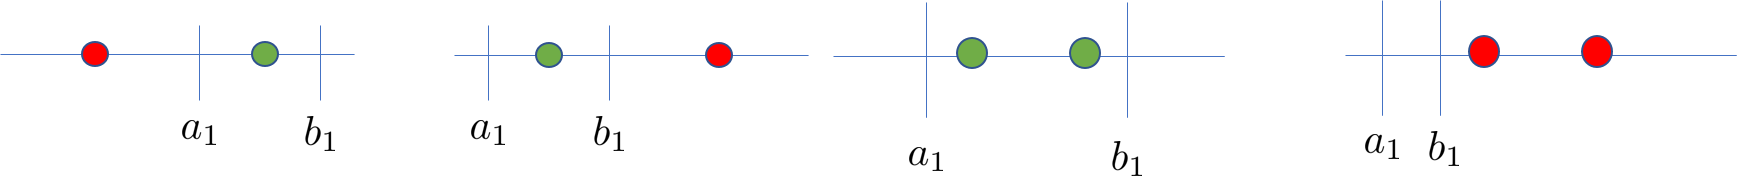
\includegraphics[scale=0.5]{q_1_a_augmented}
	\caption{$I_1$ can shatter 2 points}
\end{figure}
\\
But it cannot shatter 3 points on real line in the following configuration:
\begin{figure}[h!]
	\centering
	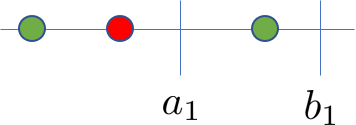
\includegraphics[scale=0.5]{q1_a_proof}
	\caption{$I_1$ cannot shatter 3 points}
\end{figure}
\subsection*{Solution 1.b}
$I_2$ is denoted by union of two closed intervals i.e. $[a_1, b_1] \cup [a_2, b_2]\in \mathbb{R}$. VC-dimension of $I_2$ is $VC(I_2) = 4$.
\subsubsection*{Proof}
union of two closed intervals i.e. $[a_1, b_1] \cup [a_2, b_2]$ can shatter 4 points on real line as shown below. For clarity, all the combinations are not shown:
\begin{figure}[h!]
	\centering
	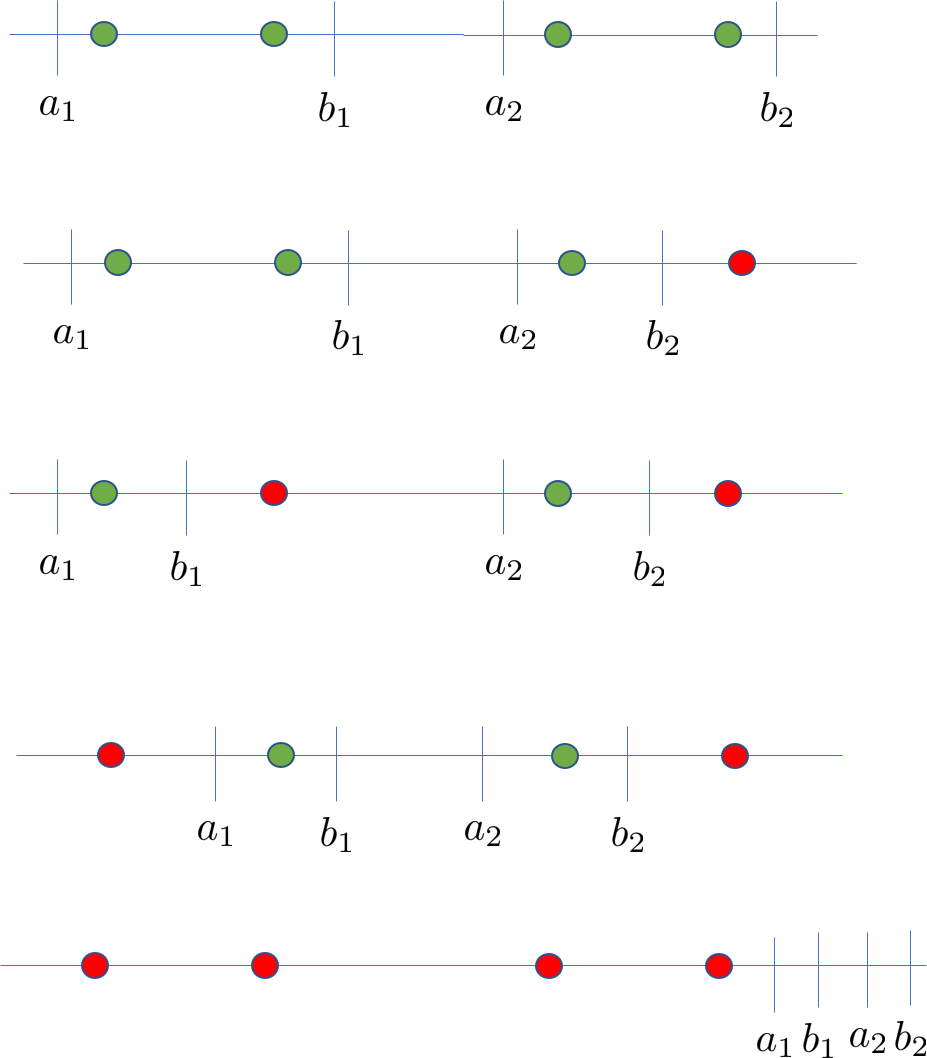
\includegraphics[scale=0.4]{q1_b}
	\caption{$I_2$ can shatter 4 points}
\end{figure}
\newpage
But it cannot shatter 5 points on real line in the following configuration:
\begin{figure}[h!]
	\centering
	
\includegraphics[scale=0.5]{q1_b_proof}
	\caption{$I_2$ cannot shatter 5 points}
\end{figure}
\subsection*{Solution 1.c}
$I_K$ is denoted by union of $K$ closed intervals i.e. $[a_1, b_1] \cup [a_2, b_2] \cup \ldots \cup [a_K, b_K] \in \mathbb{R}$. VC-dimension of $I_K$ is $VC(I_K) = 2K$.
\subsubsection*{Proof}
As any single closed interval can shatter 2 points, union of $K$ such disjoint intervals will be able to shatter $2\times K$ points. But any alternate combination of $2K+1$ negative and positive samples cannot be shattered by union of $K$ disjoint intervals. In case of overlapped intervals, the union can be considered as a single closed interval and therefore, the number of points it can shatter will be always less than disjoint intervals.